\section{Related Work}

% \begin{figure}[htbp]
%     \centering
%     \resizebox{0.98\textwidth}{!}{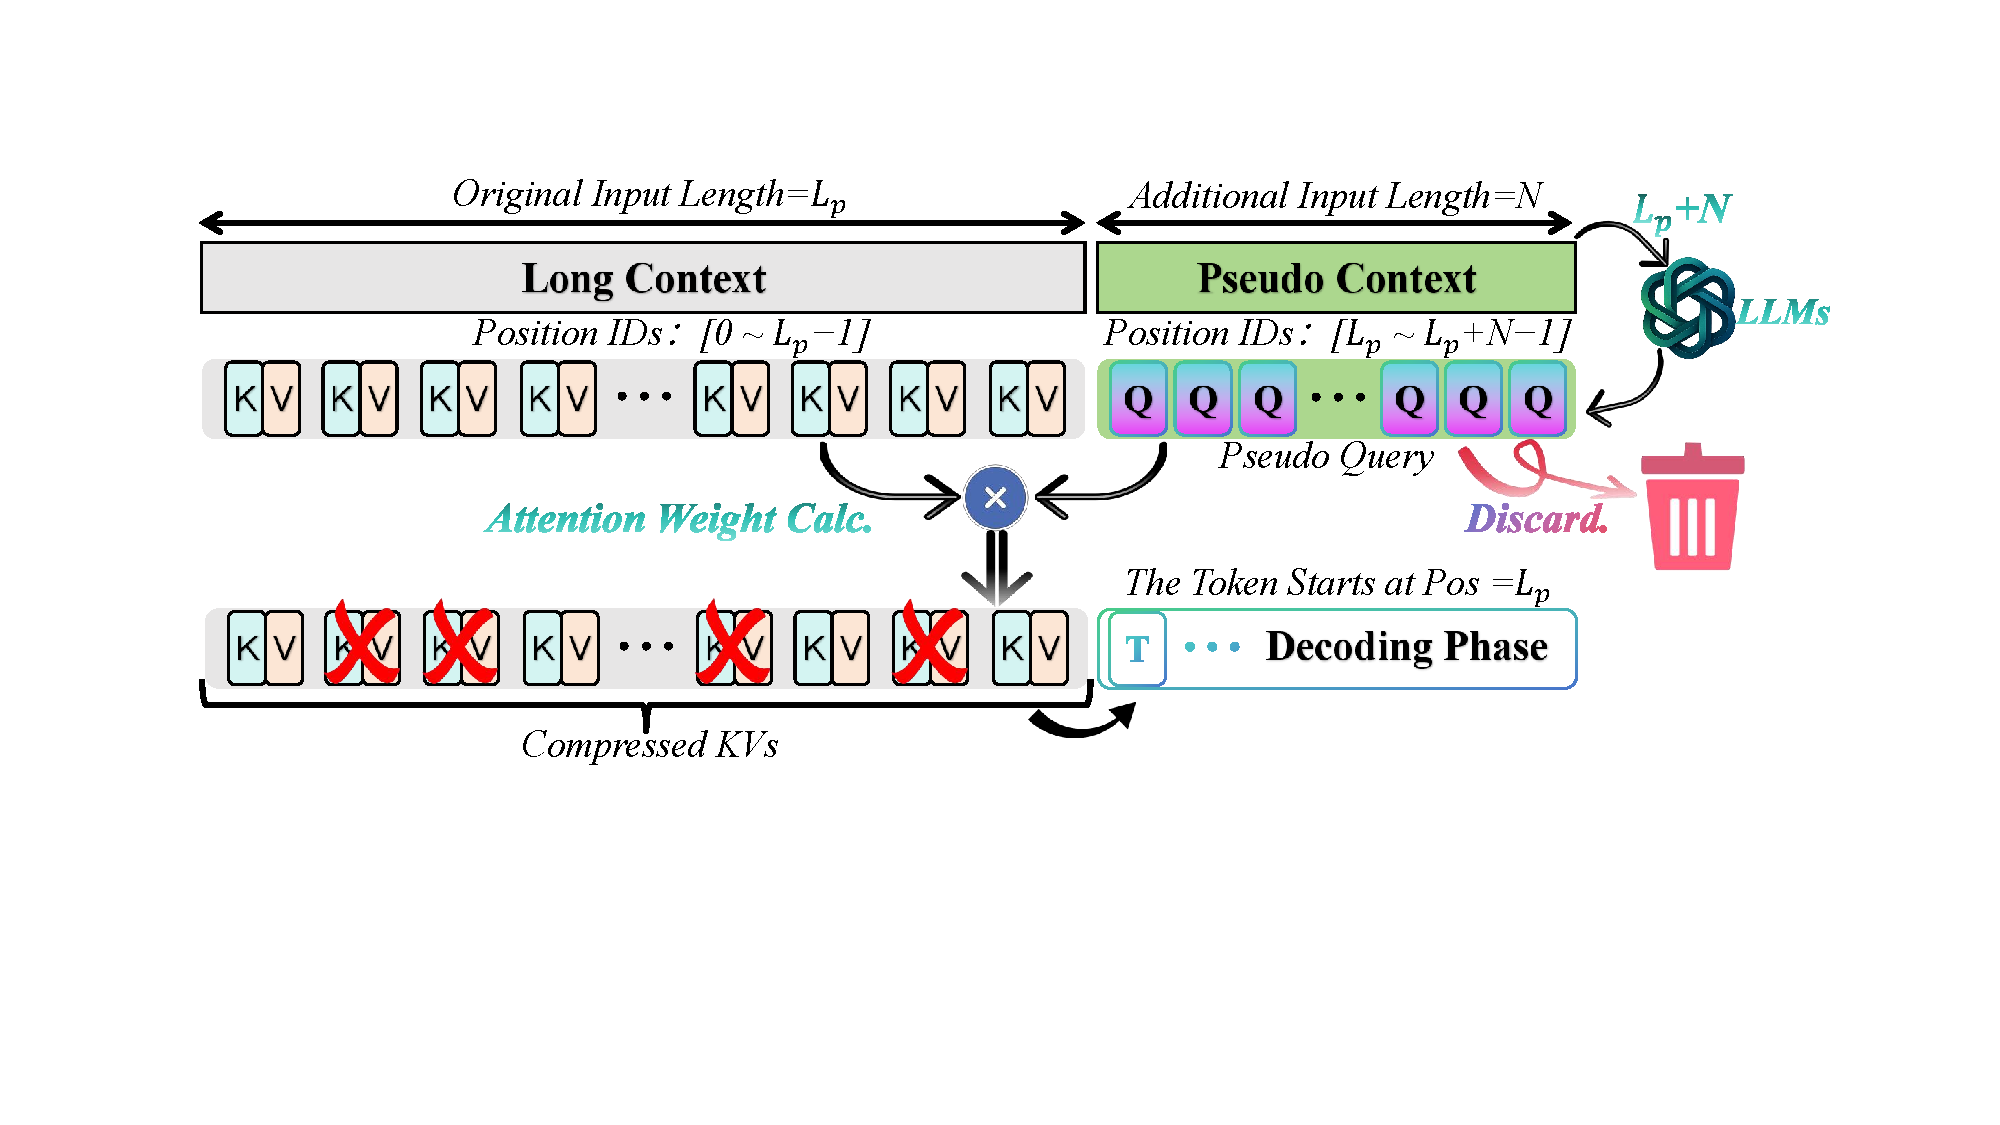
\includegraphics{images/method.pdf}} % 强制调整大小
%     \caption{An overview of DapQ.}
%     \label{fig:DapQ}
%     \vspace{-18pt}
% \end{figure}

\paragraph{Long-Context LLMs.} The growing demand for LLMs to process long contexts intensifies computational and memory challenges. Prior works address these issues through specialized fine-tuning \citep{longlora} and extending effective context windows via refined positional encodings, such as interpolation and extrapolation \citep{Interpolation,ntk}. To mitigate computational overhead, sparse attention and linear attention have been widely explored \citep{reformer,longformer,linformer}. Beyond traditional Transformer, novel architectures like State-Space Models (SSMs) \citep{longmamba,SSMs} provide linear complexity solutions for processing long sequences. Additionally, memory optimization techniques, such as KV cache compression \citep{streamingllm,snapkv} and memory offloading \citep{hcattention,deepspeed}, have been developed. These multifaceted techniques collectively advance LLMs' capabilities in handling ultra-long sequence tasks.


% \begin{table}[htbp]
% \centering
% \caption{Query Similarity Comparison under Different Conditions}
% \label{tab:query_similarity}
% \resizebox{\textwidth}{!}{%
% \begin{tabular}{c >{\raggedright\arraybackslash}p{9cm} >{\raggedright\arraybackslash}p{6cm} c c}
% \toprule
% \textbf{Experiment} & \textbf{Content Similarity} & \textbf{Positional Similarity} & \textbf{Post ROPE} & \textbf{Re ROPE} \\
% \midrule
% SC \& SP 
% & Same\textcolor{gray}{("The report discusses the Federal……Airport Improvement Program (AIP). The program")} 
% & Same\textcolor{gray}{(4424,4425,4426……4453,4454,4455)} 
% & \textcolor{green}{1.0000} & \textcolor{green}{1.0000} \\
% \addlinespace
% DC \& SP 
% & Different\textcolor{gray}{("Sorry, I don't know. Sorry, I don't know. Sorry, I don't know. Sorry, I don't know. Sorry, I")} 
% & Same\textcolor{gray}{(4424,4425,4426……4453,4454,4455)} 
% & \textcolor{green}{0.7238} & \textcolor{green}{0.7238} \\
% \addlinespace
% SC \& DP 
% & Same\textcolor{gray}{("The report discusses the Federal……Airport Improvement Program (AIP). The program")} 
% & Different\textcolor{gray}{(0,1,2……29,30,31)} 
% & \textcolor{red}{0.3267} & \textcolor{green}{0.7913} \\
% \addlinespace
% DC \& DP 
% & Different\textcolor{gray}{("Sorry, I don't know. Sorry, I don't know. Sorry, I don't know. Sorry, I don't know. Sorry, I")} 
% & Different\textcolor{gray}{(0,1,2……29,30,31)} 
% & \textcolor{red}{0.3522} & \textcolor{green}{0.7434} \\
% \bottomrule
% \end{tabular}%
% }
% \end{table}

\begin{table*}[t]
\centering
\resizebox{\textwidth}{!}{%
\begin{tabular}{c >{\raggedright\arraybackslash}p{8.5cm} >{\raggedright\arraybackslash}p{6.5cm} c c}
\toprule
\textbf{Experiment} & \textbf{Content Similarity} & \textbf{Positional Similarity} & \textbf{Post ROPE} & \textbf{Pre ROPE} \\
\midrule
% 第一行：其他列跨2行合并
\multirow{2}{*}{SC \& SP} 
& Same\textcolor{gray}{(\enquote{The report discusses the Federal……Airport Improvement Program (AIP). The program})} 
& \multirow{2}{*}{Same\textcolor{gray}{(4424,4425,4426……4453,4454,4455)}} 
& \multirow{2}{*}{\textcolor{green}{1.0000}} & \multirow{2}{*}{\textcolor{green}{1.0000}} \\
\addlinespace
% 第二行：其他列跨2行合并
\multirow{2}{*}{DC \& SP} 
& Different\textcolor{gray}{(\enquote{Sorry, I don't know. Sorry, I don't know. Sorry, I don't know. Sorry, I don't know. Sorry, I})} 
& \multirow{2}{*}{Same\textcolor{gray}{(4424,4425,4426……4453,4454,4455)}} 
& \multirow{2}{*}{\textcolor{green}{0.7238}} & \multirow{2}{*}{\textcolor{green}{0.7238}} \\
\addlinespace
% 第三行：其他列跨2行合并
\multirow{2}{*}{SC \& DP} 
& Same\textcolor{gray}{(\enquote{The report discusses the Federal……Airport Improvement Program (AIP). The program})} 
& \multirow{2}{*}{Different\textcolor{gray}{(0,1,2……29,30,31)}} 
& \multirow{2}{*}{\textcolor{red}{0.3522}} & \multirow{2}{*}{\textcolor{green}{0.7913}} \\
\addlinespace
% 第四行：其他列跨2行合并
\multirow{2}{*}{DC \& DP} 
& Different\textcolor{gray}{(\enquote{Sorry, I don't know. Sorry, I don't know. Sorry, I don't know. Sorry, I don't know. Sorry, I})} 
& \multirow{2}{*}{Different\textcolor{gray}{(0,1,2……29,30,31)}} 
& \multirow{2}{*}{\textcolor{red}{0.3267}} & \multirow{2}{*}{\textcolor{green}{0.7434}} \\
\bottomrule
\end{tabular}%
}
\vspace{-8pt}
\caption{Query similarity comparison under different content and position conditions. Post ROPE denotes similarity after ROPE has been applied to query vectors. Pre ROPE indicates similarity measured before ROPE application.}
\label{table:query_similarity}
\vspace{-8pt}
\end{table*}

\begin{figure*}
    \centering
    % 第一张子图及图注
    \begin{subfigure}[t]{0.47\textwidth}
        \centering
        \resizebox{\textwidth}{!}{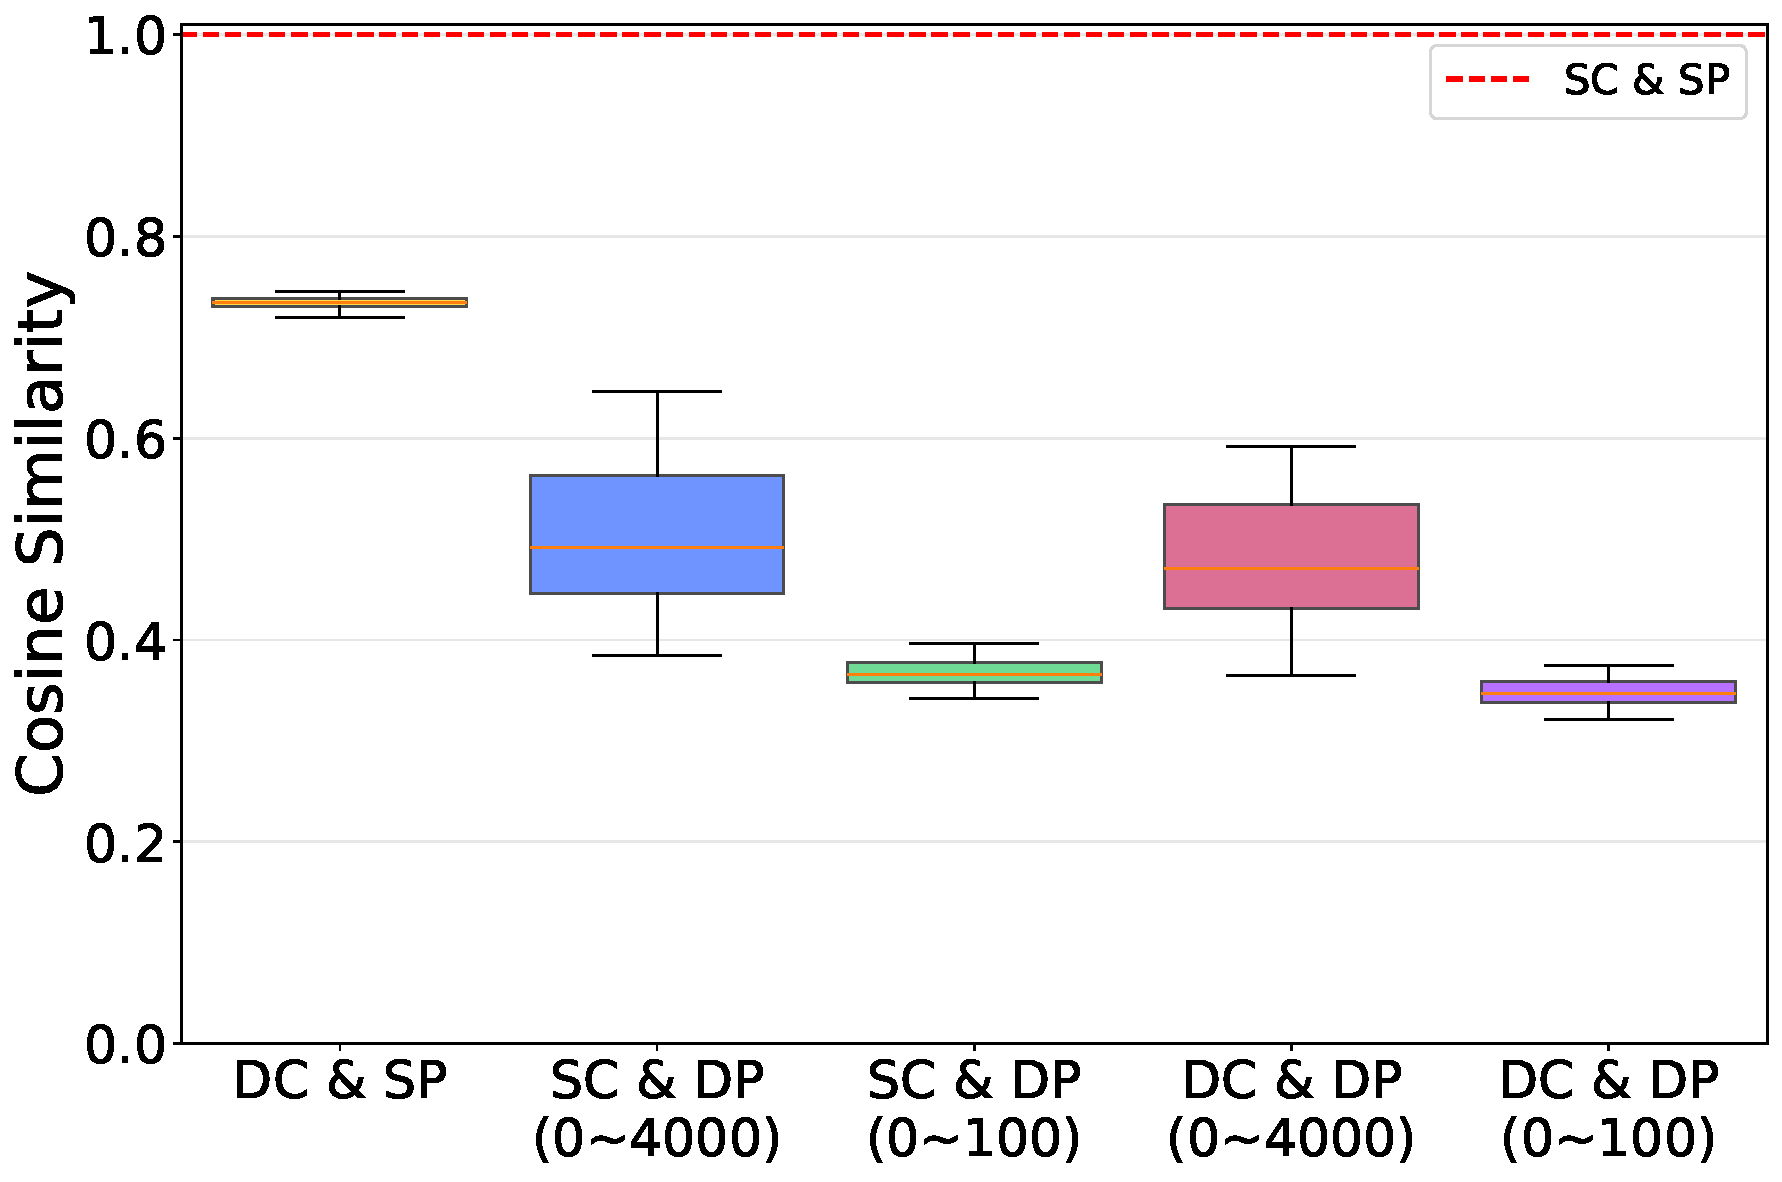
\includegraphics{images/similarity_boxplot.pdf}}
        % \caption{Boxplot of query similarity distributions.}  % 第一张图的图注
        \caption{}  % 第一张图的图注
        \label{fig:query_similarity_boxplot}
    \end{subfigure}
    \hspace{0.5cm}  % 两图间距
    % 第二张子图及图注
    \begin{subfigure}[t]{0.47\textwidth}
        \centering
        \resizebox{\textwidth}{!}{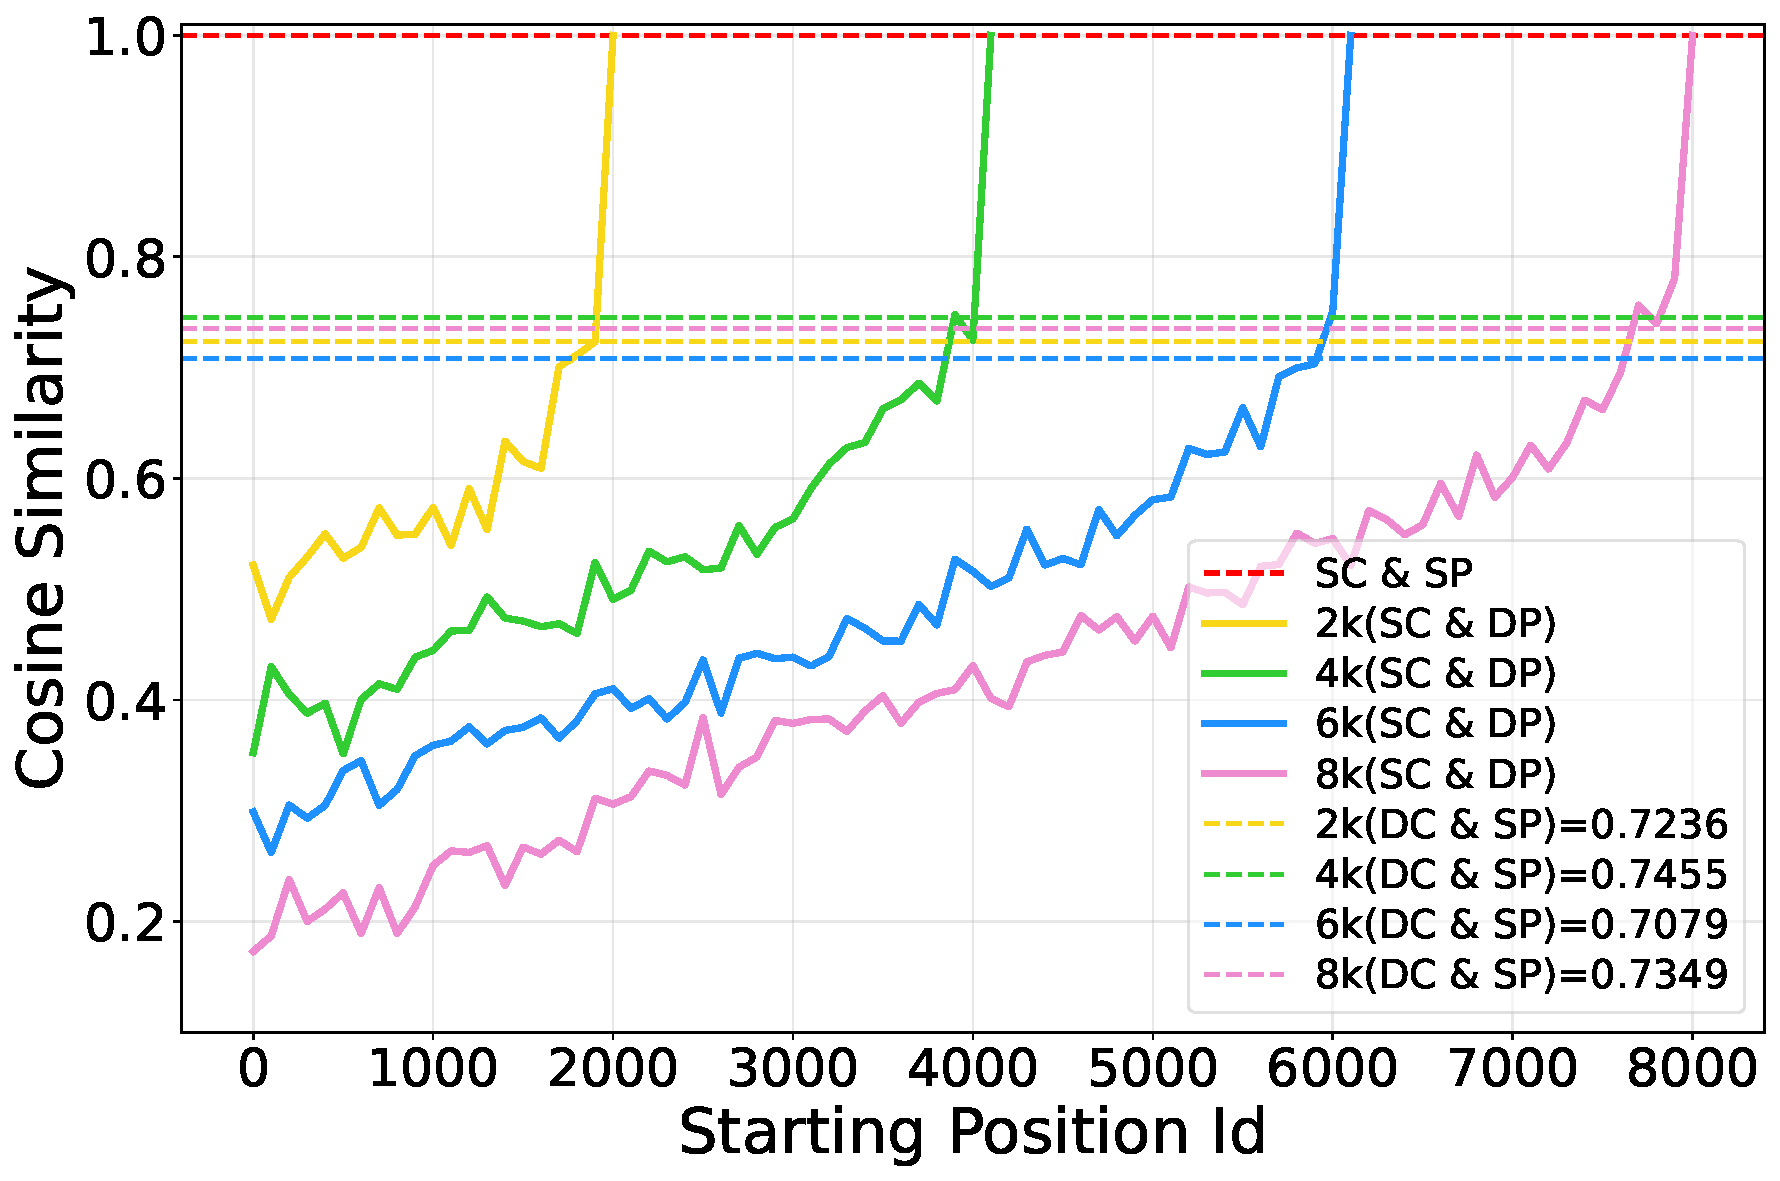
\includegraphics{images/average_similarity_curve.pdf}}
        % \caption{Curve of query similarity over offset positions.}  % 第二张图的图注
        \caption{}
        \label{fig:query_similarity_curve}
    \end{subfigure}
    \vspace{-7pt}
    % 可选总标题（概括两图内容）
    \caption{Analysis of Positional Dominance and Offset Sensitivity in Query Similarity. We set the pseudo queries of fixed length 32. (a) Boxplot of query similarity distributions for a 4k context under different content and position conditions, each aggregated from 100 independent trials. DC: pseudo-queries content is constructed by randomly sampling 32 tokens from the model's vocabulary; DP: pseudo-queries positions are assigned by randomly sampling a consecutive span of 32 index positions from the context length range [0, m] (e.g., [0, 4000]). (b) Query similarity curves over offset positions for contexts of lengths 2k, 4k, 6k, and 8k. The x-axis denotes the starting position assigned to pseudo queries (e.g., an x-axis value of 3500 corresponds to position IDs $3500\sim3531$).}
    % \caption{Analysis of Positional Dominance and Offset Sensitivity in Query Similarity. (a) Query similarity distributions from large-scale sampling of content and position variations. DC: pseudo-queries content is constructed by randomly sampling 32 tokens from tokenizer's vocabulary; DP: pseudo-queries positions are assigned by randomly sampling consecutive span of 32 indices from [0, m]. (b) Similarity decay with positional offset across context lengths(2k-8k). Similarity decay with positional offset across context lengths.We sample instances from GovReport with input lengths of 2k, 4k, 6k, and 8k. The x-axis indicates the starting position of the 32-token pseudo-queries (e.g., 2500 corresponds to position IDs 2500–2531).  }

    \vspace{-14pt}
\end{figure*}

%Experiment select an example (input token length: 4424) from the GovReport dataset for summarization task. True queries comprise the first 32 output tokens from LLaMA-3-8B-Instruct with content \textcolor{gray}{"The report discusses the Federal Aviation Administration's (FAA) state block grant pilot program, which is part of its Airport Improvement Program (AIP). The program"} at positions \textcolor{gray}{4424-4455}. We artificially synthesized a 32-length context with \textcolor{gray}{"Sorry, I don't know. Sorry, I don't know. Sorry, I don't know. Sorry, I don't know. Sorry, I"}. Pseudo queries vary in both content (correct:\textcolor{gray}{"The report discusses..."} or incorrect: \textcolor{gray}{"Sorry, I don't know..."}) and position assignments (correct: \textcolor{gray}{4424-4455} or incorrect: \textcolor{gray}{0-31}). Results represent cosine similarity between pseudo queries and true queries under Post-ROPE and Re-ROPE conditions.


%\caption{Experimental setup using a GovReport summarization example (input length: 4424) with LLaMA-3-8B-Instruct. True queries comprise the first 32 output tokens with content \textcolor{gray}{"The report discusses the Federal Aviation Administration's (FAA) state block grant pilot program, which is part of its Airport Improvement Program (AIP). The program"} at positions \textcolor{gray}{4424-4455}，same as Table 1' experimental setting. Pseudo-queries use random token sequences from the tokenizer vocabulary as semantic content. Position assignments vary: correct positions (\textcolor{gray}{4424-4455}), wide-range incorrect positions (32 consecutive positions randomly selected from 0-4000), and narrow-range incorrect positions (32 consecutive positions from 0-100). Dashed lines indicate the specific SC&DP (0.3267) and DC&DP (0.3522) Post-ROPE similarity values from Table 1 for reference.}”.Each configuration was tested over 50 times with averaged results.Statistical results are based on 50 trials per configuration.

\paragraph{KV Cache Compression.} KV cache compression is crucial for enhancing the inference efficiency and deployability of LLMs, particularly in resource-constrained scenarios. Various methods have been developed to reduce KV cache memory footprint. Token eviction strategies aim to retain only the most important tokens based on metrics like attention scores \citep{snapkv,h2o}, positional heuristics \citep{streamingllm}, special tokens \citep{gemodel,sepllm}, or norm-based criteria \citep{simple}. Quantization \citep{kivi,kvquant} reduces memory by storing less important KV pairs with lower precision, some approaches even achieving sub-2-bit quantization via token-aware and channel-aware techniques. Sharing-based approaches deliver memory savings and accelerate inference through head-wise sharing \citep{mqa,gqa}, inter-layer sharing \citep{sun2024you,wu2024layer,brandon2024reducing}, or prefix sharing across sequences \citep{hydragen,relayattention}. Low-rank decomposition \citep{gear,palu} projects KV cache into lower-dimensional spaces to exploit inherent redundancy, as demonstrated by the Multi-Head Latent Attention \citep{deepseekv3} of DeepSeek, which reduces cache size through low-rank compression and decoupled RoPE while preserving model performance. KV merging \citep{keepkv,homogeneous} employs attention-pattern similarity or reparameterization to merge similar semantic information, achieving effective compression with minimal performance loss.





